\documentclass{beamer}

\title{Visual Workflow Automation Tools}
\subtitle{\texorpdfstring{\tiny{\href{https://invent.kde.org/cschumac/feep/-/tree/master/tools/presentation_Visual_Workflow_Automation_Tools}{https://invent.kde.org/cschumac/feep/-/tree/master/\\tools/presentation\_Visual\_Workflow\_Automation\_Tools}}}{}}
\author{David Hurka}
\date{2021-10-08}

\begin{document}
    \begin{frame}
        \titlepage
    \end{frame}

    \begin{frame}
        \frametitle{xdotool}
        \framesubtitle{\url{https://www.semicomplete.com/projects/xdotool}}

        Command line interface to XTEST

        \begin{columns}
            \begin{column}{5cm}
                \begin{itemize}
                    \item Send input events
                    \item Manipulate windows
                \end{itemize}

                \vskip 1em

                \begin{itemize}
                    \item X
                    \item Same desktop
                \end{itemize}
            \end{column}

            \begin{column}{7cm}
                \begin{semiverbatim}
                    xdotool key ctrl+o

                    sleep 1

                    xdotool type "20yearsofKDE.pdf"

                    sleep 1

                    xdotool key Return
                \end{semiverbatim}
            \end{column}
        \end{columns}
    \end{frame}

    \begin{frame}
        \frametitle{Xnee}
        \framesubtitle{\url{https://savannah.gnu.org/projects/xnee/}}

        Library and tool for GUI testing

        \vskip 1em

        \begin{itemize}
            \item Record input events to file
            \item Replay from file to multiple X sessions
            \item Compress mouse events
        \end{itemize}

        \vskip 1em

        \begin{itemize}
            \item X
        \end{itemize}

        \vskip 1em

        \begin{semiverbatim}
            6,2,0,0,0,37,0,350337,3,Virtual core keyboard

            7,6,992,614,0,0,0,462213,13,'TPPS/2 IBM TrackPoint'
        \end{semiverbatim}
    \end{frame}

    \begin{frame}
        \frametitle{PyAutoGUI}
        \framesubtitle{\url{https://pypi.org/project/PyAutoGUI/}}

        Library for GUI automation

        \vskip 1em

        \begin{itemize}
            \item Send input events
            \item Make screenshots
            \item Locate images
        \end{itemize}

        \vskip 1em

        \begin{itemize}
            \item X
            \item Same desktop, only primary screen
        \end{itemize}

        \vskip 1em

        \begin{semiverbatim}
            b = pyautogui.locateOnScreen('button.png')

            pyautogui.click(center(b))
        \end{semiverbatim}
    \end{frame}

    \begin{frame}
        \frametitle{Atbswp / Automate the boring stuff with Python}
        \framesubtitle{\url{https://github.com/rmpr/atbswp}}

        wxPython toolbar

        \begin{columns}
            \begin{column}{5cm}
                \begin{itemize}
                    \item Record and replay macros
                    \item Export as Python script
                \end{itemize}

                \vskip 1em

                \begin{itemize}
                    \item X (PyAutoGUI)
                    \item Wayland announced
                \end{itemize}
            \end{column}

            \begin{column}{5cm}
                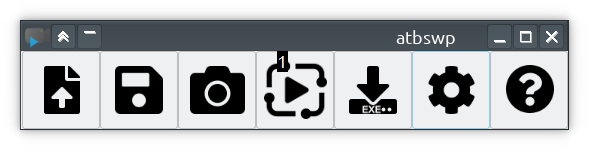
\includegraphics[width=5cm]{Images/atbswp_screenshot.png}
            \end{column}
        \end{columns}
    \end{frame}

    \begin{frame}
        \frametitle{Actiona}
        \framesubtitle{\url{https://actiona.tools/}}

        GUI application for visual workflow automation

        \begin{columns}
            \begin{column}{4cm}
                \begin{itemize}
                    \item Send input events
                    \item Drag\&drop editor for workflows
                    \item JavaScript scripting
                \end{itemize}

                \vskip 1em

                \begin{itemize}
                    \item X
                    \item Same desktop
                \end{itemize}
            \end{column}

            \begin{column}{7cm}
                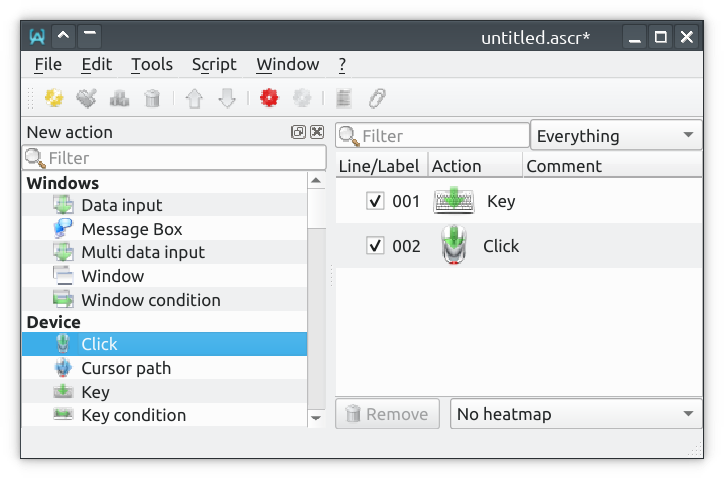
\includegraphics[width=7cm]{Images/actiona_screenshot.png}
            \end{column}
        \end{columns}
    \end{frame}

    \begin{frame}
        \frametitle{Sikulix}
        \framesubtitle{\url{https://sikulix.com}}

        GUI application for visual workflow automation

        \begin{columns}
            \begin{column}{5cm}
                \begin{itemize}
                    \item Send input events
                    \item IDE with inline thumbnail display
                    \item JPython scripting
                    \item Make screenshots
                    \item Locate text and images
                \end{itemize}

                \vskip 1em

                \begin{itemize}
                    \item X
                    \item Same desktop
                \end{itemize}
            \end{column}

            \begin{column}{7cm}
                \begin{figure}
                    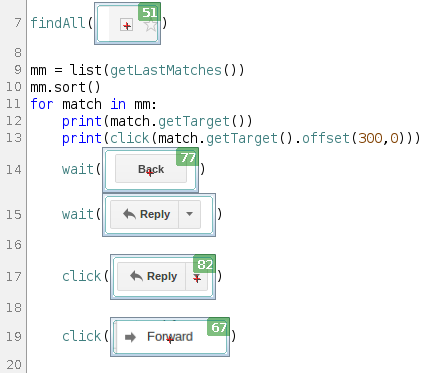
\includegraphics[width=7cm]{Images/sikulix_example.png}
                    \tiny{\url{https://wiki.sydarkivera.se/wiki/Fil:Sikulix.png}}
                \end{figure}
            \end{column}
        \end{columns}
    \end{frame}

    \begin{frame}
        \frametitle{Squish}
        \framesubtitle{\url{https://www.froglogic.com/squish/}}

        Automatic GUI test suite (proprietary)

        \vskip 1em

        \begin{itemize}
            \item Record and send input \& toolkit events
            \item Locate text and images
        \end{itemize}

        \vskip 1em

        \begin{itemize}
            \item GUI toolkit
            \item VNC
        \end{itemize}
    \end{frame}

    \begin{frame}
        \frametitle{Eggplant Functional}
        \framesubtitle{\url{http://docs.eggplantsoftware.com/ePF/gettingstarted/epf-getting-started-eggplant-functional.htm}}

        Automatic GUI test suite (proprietary)

        \vskip 1em

        \begin{itemize}
            \item Record and send input events
            \item Locate text and images
        \end{itemize}

        \vskip 1em

        \begin{itemize}
            \item VNC
            \item RDP
        \end{itemize}
    \end{frame}

    \begin{frame}
        \frametitle{PuloversMacroCreator}
        \framesubtitle{\url{https://macrocreator.com}}

        GUI application for visual workflow automation

        \vskip 1em

        \begin{itemize}
            \item Record and send input events
            \item IDE for AutoHotkey scripts
            \item Locate images
        \end{itemize}

        \vskip 1em

        \begin{itemize}
            \item Windows (AutoHotkey)
        \end{itemize}

        \begin{figure}
            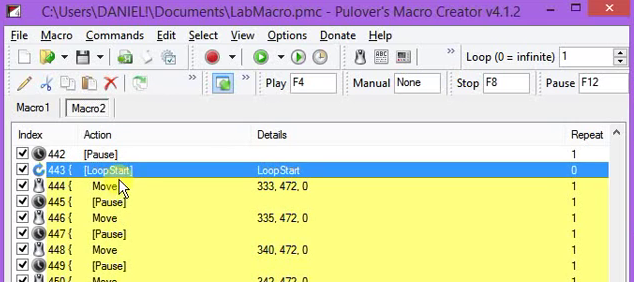
\includegraphics[height=3cm]{Images/pulovers_macro_creator_example.png}
            \tiny{\url{https://www.youtube.com/watch?v=nP6qE5gwbfU}}
        \end{figure}
    \end{frame}

    \begin{frame}
        \frametitle{WinAutomation / Microsoft Power Automate Desktop}
        \framesubtitle{\url{https://docs.microsoft.com/en-us/power-automate/desktop-flows/}}

        “Robotic process automation”

        \begin{columns}
            \begin{column}{6cm}
                \begin{itemize}
                    \item Record and send input events
                    \item Locate images
                    \item Manipulate windows
                \end{itemize}

                \vskip 1em

                \begin{itemize}
                    \item Windows
                \end{itemize}
            \end{column}

            \begin{column}{6cm}
                \begin{figure}
                    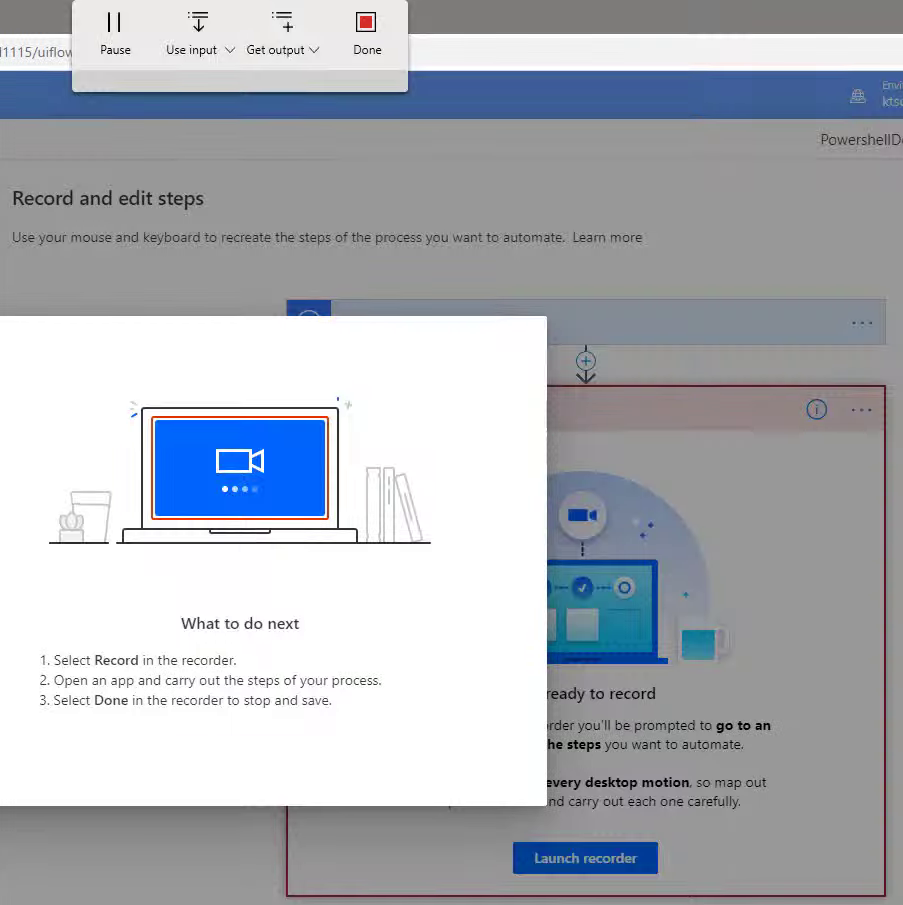
\includegraphics[width=6cm]{Images/power_automate_screenshot.png}
                    \tiny{\url{https://www.youtube.com/watch?v=s-Z-Y4cErAE}}
                \end{figure}
            \end{column}
        \end{columns}
    \end{frame}
\end{document}
